\documentclass[11pt]{report}

\usepackage{graphicx}
\usepackage{amssymb}
\usepackage{amsbsy}
\usepackage{float}
\usepackage{amsmath}
\usepackage{pifont}
\usepackage{multirow}
\usepackage{setspace}
\usepackage{grffile}
\usepackage{verbatim}
\usepackage[top=50px,right = 60px,left = 60px, bottom = 60px]{geometry}

\usepackage[shortlabels]{enumitem}
\usepackage{tikz}
\usepackage{caption}
\captionsetup[figure]{slc=off}
\usepackage{subcaption}
\usepackage{listings}
\usepackage{threeparttable}%

\usepackage{titlesec}
\titleformat{\chapter}[display]   
{\normalfont\huge\bfseries}{\chaptertitlename\ \thechapter}{10pt}{\Huge}   
\titlespacing*{\chapter}{0pt}{-30pt}{10pt}



\onehalfspacing

\newcommand{\cmark}{ \color{green} \ding{51}}%
\newcommand{\xmark}{ \color{red} \ding{55}}%

\newcommand{\psibold}{\mbox{\boldmath$\psi$}}
\newcommand{\nablabold}{\mbox{\boldmath$\nabla$}}
\newcommand{\sigmabold}{\mbox{\boldmath$\sigma$}}

\renewcommand{\thetable}{\Roman{table}}

\setlength{\parskip}{2ex}
\setlength{\parindent}{0pt}


\def\MM#1{\boldsymbol{#1}}




\newcommand{\reporttitle}{Calibration of models of cardiac electrophysiology using machine learning}
\newcommand{\reportauthor}{Benjamin Marchand}
\newcommand{\reporttutors}{Chris Cantwell, Charles Houston}
\newcommand{\reporttype}{Master Thesis}
\newcommand{\cid}{01605579}
\newcommand{\stdwidth}{10cm}



\usepackage[backend = biber]{biblatex}
\addbibresource{mybibliography.bib}

\begin{document}

% front page
\begin{titlepage}

\newcommand{\HRule}{\rule{\linewidth}{0.5mm}} % Defines a new command for the horizontal lines, change thickness here


%----------------------------------------------------------------------------------------
%	LOGO SECTION
%----------------------------------------------------------------------------------------


\includegraphics[width = 4cm]{./figures/imperial}\\[0.5cm] 

\begin{center} % Center remainder of the page

%----------------------------------------------------------------------------------------
%	HEADING SECTIONS
%----------------------------------------------------------------------------------------
\textsc{\LARGE \reporttype}\\[1.5cm] 
\textsc{\Large Imperial College London}\\[0.5cm] 
\textsc{\large Department of Aeronautics}\\[0.5cm] 
\textsc{\Large MSc Advanced Computational Methods for Aeronautics, Flow Management and Fluid-Structure Interaction}\\[0.5cm] 

%----------------------------------------------------------------------------------------
%	TITLE SECTION
%----------------------------------------------------------------------------------------

\HRule \\[0.4cm]
{\Large{\textbf{\reporttitle}}}\\ % Title of your document
\HRule \\[2cm]
\end{center}
%----------------------------------------------------------------------------------------
%	AUTHOR SECTION
%----------------------------------------------------------------------------------------

%\begin{minipage}{0.4\hsize}
\begin{flushleft} \large
\textit{Author:}\\
\reportauthor~(CID: \cid) % Your name
\end{flushleft}

\begin{flushleft} \large
\textit{Tutors:}\\
\reporttutors % the names of the tutors
\end{flushleft}

\vspace{2cm}
\makeatletter
Date: September 13, 2019

\vfill % Fill the rest of the page with whitespace



\makeatother


\end{titlepage}



\begin{abstract}
    With the increasing complexity of the human atrial cell models and the advent of deep learning, most recent papers tend to focus on using cutting-edge algorithms to keep improving models of the human atrial cell. However those algorithms induce the loss of the interpretability of the parameters of the model and limit their ability to generalise to other sets of data. Moreover those algorithms don't allow the assessment of the uncertainty around the values of the parameters.
    This report focuses on using a Bayesian algorithm called the Approximate Bayesian Computation Sequential Monte Carlo (ABCSMC) in order to assess the existing models of the human atrial cell and understand the limitations of the current models. Indeed this statistical method allows to infer the parameter's value as well as uncertainty around those values. The investigated human atrial cell models are the Nygren \cite{Nygren1998} model, the Courtemanche \cite{Courtemanche1998} model and a standardised model which leads to structural identifiability and parameters identifiability results on those models. A focus on the Sodium channel and on the Calcium channel will be made and regarding those two channels. This work shows that a standard model with fewer parameters than more complex models ,as the Nygren \cite{Nygren1998} or Courtemanche \cite{Courtemanche1998} one, is enough to correctly reproduce experimental data from several papers.
\end{abstract}

\tableofcontents



\chapter{Introduction}

Clinics need more and more mathematical models to to have better ways to heal patients inducing a need to have a better precision on the models and uncertainty around the values of parameters that are found. Those are needed to understand the limitations of the model. Moreover, experiments on the human heart are complex to realise which makes the human atrial cells (cardiac cells) important to model. To understand the models that will be presented in this report, one must understand first the global picture. The contraction of the heart is due to an electrical wave propagating through the heart, heart arrhythmia for instance relates to a problem of propagation of this electrical wave. Now the fact that the heart contracts only means that the cells contract and human atrial cells contract because there is a flux of ions through ion-specific channels across the cell membrane. An Action Potential (AP) is represented on figure \ref{fig:AP} : it corresponds to the change in voltage across the cell membrane. The action potential is therefore the propagating electrical wave which controls coordinated contraction of the heart.
As seen on the figure \ref{fig:AP}, it is caused by the entrance and exit of ions through channels : the depolarisation is caused by the entrance of sodium ions and makes the voltage increase very quickly. Then the repolarisation takes place : the potassium goes out of the cell while calcium comes in until the resting potential is reached again.

\begin{figure}[H]
    \centering
    \begin{measuredfigure}
    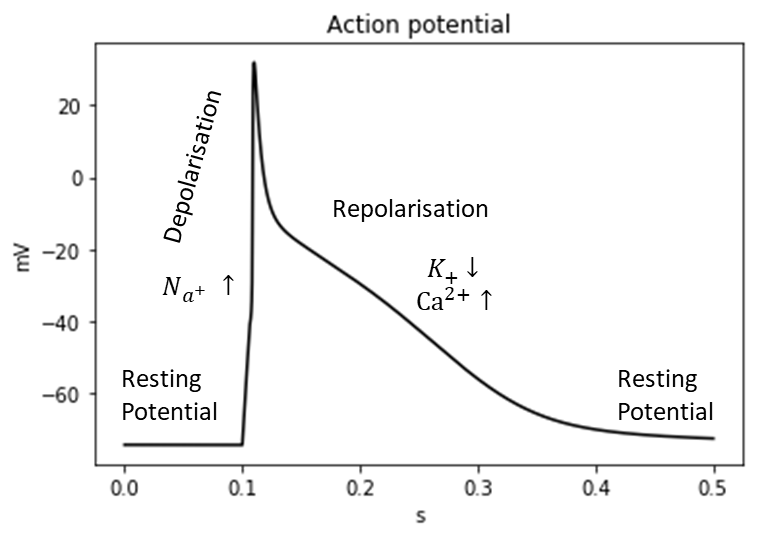
\includegraphics[scale = 0.75]{figures/AP.png}
    \captionsetup{singlelinecheck = false, format= hang, justification=raggedright, font=footnotesize, labelsep=space}
	\caption{Example of an action potential plotted against time}
	\end{measuredfigure}
      \addtocounter{figure}{-1}
      \phantomcaption
	\label{fig:AP}
\end{figure}



The human atrial cell models then try to correctly model the cell and reproduce the action potential according to experiments that were conducted twenty years ago. The quality and robustness of those models was hard to quantify because the values found for the parameters were not associated with any uncertainty : the usual fitting technique at the time was the least square method \cite{Sakakibara1992}. 

Yet the statistics have developed and now uncertainty and identifiability can be captured by new fitting algorithms and one will be developed in the Method section. This report will analyse two main channels of the human atrial cell : the Sodium channel ($I_{Na}$) and the Calcium channel ($I_{Ca L}$). The objectives of the report are to answer the following questions :
Can the existing human atrial models capture the experimental data ?
Can we use a standardised model to capture the same experimental data with fewer parameters ?
In order to answer those questions, the identifiability, uncertainty, biologic variability of the parameters of those models will be quantified.
The next chapter will define the notions presented here and introduce the workflow of the project.





\chapter{Methods}

\section{Method workflow}

The workflow followed through the project is explained in this section, and the particular items presented will be detailed in the next sections.
Here is the method applied :

\begin{itemize}

    \item Firstly, a model was selected from the modeling papers. Then regarding the chosen channel, the equations of the other channels were removed to only keep in the code the studied channel.
    
    \item Secondly, experimental data about the chosen channel was extracted from one or several papers. The experimental data here represent the data points from the figures of the results of experiments, the experimental protocols applied to obtain those results and the external conditions during the experimentations such as the concentration and the temperature.

    
    \item Afterwards, the fitting algorithm was ran on the experiments separately in order to assess the structural identifiability of the model. The structural identifiability is about the structure of the equations of the model according to a data set : a model is structurally identifiable if there exists a set of parameters that can make the model fit to the data. On Figure \ref{fig:StructuralIdentifiabilityExample} is represented an example of structural unidentifiability and identifiability : the linear model cannot fit the data generated by $y = (x-3)^2$ whereas a quadratic model can.
    
\begin{figure}[H]
    \centering
    \captionsetup{singlelinecheck = false, format= hang, justification=centerlast, font=footnotesize, labelsep=space}
    \begin{subfigure}[b]{0.49\textwidth}
    \centering
        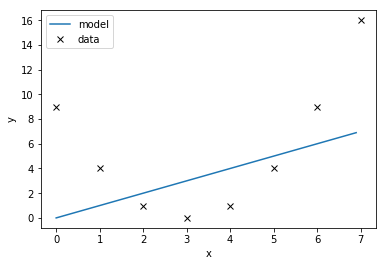
\includegraphics[width=\linewidth]{figures/structuralUnidentifiability.png}
        \caption{Structural unindentifiabililty : the model here is linear : $y=ax$ and the data is u-shaped : $y = (x-3)^2$. The model will not correctly fit the data, it's not complex enough.}
    \end{subfigure}
    \begin{subfigure}[b]{0.49\textwidth}
    \centering
        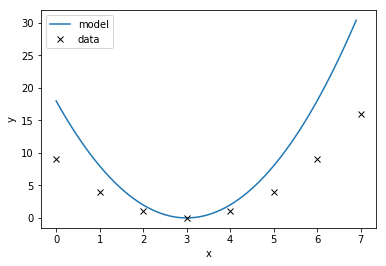
\includegraphics[width=\linewidth]{figures/structuralIdentifiability.png}
        \caption{Structural indentifiabililty : the model here is quadratic : $y=a(x-x_0)^2$ and the data is u-shaped : $y = (x-3)^2$. The model can fit the data correctly after running the fitting algorithm.}
    \end{subfigure}
    ~
    \caption{Example of structural unindentifiabililty on the left and structural indentifiabililty on the right}
    \label{fig:StructuralIdentifiabilityExample}
\end{figure}
    
    \item Finally, after testing the structural identifiability of the model, the parameter identifiability is tested. The algorithm is ran on all the experiments that the model can capture (that passed the structural identifiability test) in order to infer the parameters to the model. The parameter identifiability is about the parameters of the equations of the model : Are they all necessary to the model ? Can they all be determined ? Keeping the example $y = (x-3)^2$, let the model be $y =ax^3 + b(x-c)^2 +d10^{-10} $. In this case the parameter $"a"$ is identifiable but also unnecessary to the model, and the parameter $"d"$ is unidentifiable : no matter what value it takes, it will not affect the model since it's multiplied by $10^{-10}$. This step also allows to test the model in "real" conditions, to see if it is able to reproduce the whole behaviour of the channel being modelled.

    
\end{itemize}



\section{Models}
In this section, the equations and the physics behind them will be treated. For the sake of simplicity, a standard model will be used to understand the basic equations of the current and voltage in a human atrial cell.

From a global point of view, the equation ruling the evolution of voltage across the cell membrane is:
\begin{eqnarray}
\dfrac{dV}{dt} = \dfrac{1}{-C_{m}} \sum_{j} I_{j}
\end{eqnarray}
Where $I_{j}$ represent the different ionic currents : sodium, calcium, etc. and $C_{m}$ is the membrane capacitance of the cell.

The equation (2.1) allows the computation of the voltage as function of the different current of ions flowing through the cells. This equation is important to understand how the different channels interact with each other and sum up to create the action potential. However, as it will be seen in the experiments presented after, the voltage of the cell membrane is imposed as steps, so the focus will be done on the equations that are function of the voltage ($X= f(V)$). For instance, the equations of the sodium channel are the following :

$$I_{Na} = g_{Na}(V-E_{Na})$$
$$g_{Na} = g_{Na,max}m^{3}h $$
$$\dfrac{dm}{dt} = \dfrac{m_{\infty}(V,\theta) - m}{\tau_{m}(V,\theta)}$$
$$\dfrac{dh}{dt} = \dfrac{h_{\infty}(V,\theta) - h}{\tau_{h}(V,\theta)}$$

\newpage

Where :
\begin{itemize}
    \item $g_{Na}$ is the conductance of the cell per unit area for the sodium ion.
    
    \item $E_{Na} $ represent the reversal potential of the sodium : it is the boundary potential between $I_{Na} >0$ and $I_{Na} <0$.
    
    \item $m$ is the activation gate : it's a function of time and voltage between 0 and 1 that represent the opening of the channel. 0 means that the gate is closed or not activated and 1 that the gate is fully opened or activated. It therefore controls the ionic current flowing in the cell. $m_{\infty}$ is the value $m$ takes after a time $t>>\tau_{m}$, and is also in $[0,1]$. More details about the gates will be given in a few paragraphs.
    
    \item $h$ is the inactivation gate : like the activation gate $m$ it's a function of time and voltage between 0 and 1 that represent the opening of the channel. 0 means that the gate is closed or not inactivated and 1 that the gate is open or inactivated. $h_{\infty}$ is the value $h$ takes after a time $t>>\tau_{h}$, and is also in $[0,1]$.
    
    \item The equations of $m_{\infty}$, $\tau_{m}$, $h_{\infty}$ and $\tau_{h}$ are in the appendix 1. However the most important thing to retain from those equations is that these 4 values of the model are function of the membrane voltage and are parameterised by $\theta$. $\theta$ represent in fact the concatenated vector of all the parameters for those 4 equations and other parameters if needed, depending on the equations used.
\end{itemize}
Another important point here is to understand the concept of the gates : $m$ and $h$. Those variables are important since they model the opening and closing of ion channels considered (sodium here) in the cell and interact with each other the following way (see table \ref{tab:mandhfunctionning}). Physically, the inactivation time constant $\tau_{h}$ is at least twice greater than the activation time constant $\tau_{m}$, making the opening of the channel possible if one refers to the equation $g_{Na} = g_{Na,max}m^{3}h $. Indeed, after a time $t$ verifying $ \tau_{m} << t << \tau_{h}$ (table \ref{tab:mandhfunctionning} .a), the gate $m$ has reached it's convergence value $m_{\infty}$ which depend on the voltage applied and the gate $h$ has not reached yet it's convergence value $h_{\infty}$ (which also depend on the voltage) and is still approximately equal to 1. It then allows the current to flow through the cell since both gates are non zero. On the other hand if $t >> \tau_{h}$ (table \ref{tab:mandhfunctionning} .b), then $h$ reaches $h_{\infty}$ which is likely to be close to 0 (depending on the value of the voltage imposed). Examples curves will be shown in the next section.
\begin{figure}[H]
    \centering
    \captionsetup{singlelinecheck = false, format= hang, justification=centerlast, font=footnotesize, labelsep=space}
    \begin{subfigure}[b]{0.5\textwidth}
        \begin{tabular}{|c|c|c|c|}
        \hline
        Potential applied & m(V) & h(V) & $I_{Na}$\\
        \hline
        $V_{hold}$ (initial) &  $m_{\infty}(V_{hold}) =0$   &  $h_{\infty}(V_{hold}) =1$ & 0 \\
        \hline
        $V_{step}$ &  $m_{\infty}(V_{step})> 0$   &  $h(V_{step}) = 1$  &  $\neq 0$  \\
        \hline
        $V_{test}$ &  $m_{\infty}(V_{test}) = 1$ &  $h(V_{step}) = 1$& $\neq 0$ \\
        \hline
        \end{tabular}
        \caption{Table corresponding to t verifying $ \tau_{m} << t << \tau_{h}$.}
    \end{subfigure}
    \begin{subfigure}[b]{0.5\textwidth}
        \begin{tabular}{|c|c|c|c|}
        \hline
        Potential applied & m(V) & h(V) & $I_{Na}$\\
        \hline
        $V_{step}$ &  $m_{\infty}(V_{step})> 0$ &   $h_{\infty}(V_{step}) = 0$ &   0  \\
        \hline
        $V_{test}$ & $m_{\infty}(V_{test})=1 $  &  $h_{\infty}(V_{test}) = 0$ & 0 \\
        \hline
        \end{tabular}
        \caption{Table corresponding to t verifying $t >> \tau_{h}$. }
    \end{subfigure}

    ~
    \caption{Table of the behaviour of m and h gate after imposing the corresponding voltage. (a) corresponds to the behaviour after a "short" time : $ \tau_{m} << t << \tau_{h}$. (b) corresponds to the behaviour after a long time : $t >> \tau_{h}$. The holding voltage before the step is assumed to be equal to $V_{hold}$ and the cell is at rest.}
    \label{tab:mandhfunctionning}
\end{figure}


This is the set of equations for one ion channel only, however while focusing on one channel, the others are computationally inhibited : their equations won't be taken into account. The previous set of equations is therefore representative of the ones that the code will use to run the simulations for each channel. As explained in the introduction, the project has been focused on two main ion channels : the Sodium (Na) one and Calcium (Ca) one. The sodium channel is the most important since it is the channel responsible for the depolarization of the cell and the Calcium one is responsible for the mechanical contraction of the cell.

\section{Data}

In this section the experimental data will be detailed as well as the  protocols leading to the results of those experiments.

The data was extracted from three papers : the Sakakibara paper \cite{Sakakibara1992}, the Schneider \cite{Schneider1994} paper and finally Li and Nattel's paper \cite{Li1997}. As explained the focus will be made on two ion channels and Sakakibara \cite{Sakakibara1992} as well as Schneider \cite{Schneider1994} concentrate on the first one : the sodium channel.
The third paper Li and Nattel \cite{Li1997} focuses on the L-type Calcium channel.

Those papers have been written more than twenty years ago, so the exact points of data were not available. A plot digitilizer has been used to recollect data from the plots and the curves : the x and y axis are calibrated first from a screenshot of the plot, then the points are collected and turned into ($x_{i}$,$y_{i}$) couples. Then the data was adjusted to the models using the $Q_{10}$ factor : this is a temperature adjustment that takes into account the temperature at which the experiments were conducted and the temperature for which the model were created. Here is the formula used : $y_{adjusted} = y Q_{10}^{\alpha (T_{model}-T_{exp})/10}$ where $\alpha$ takes the value $+/-1$ depending on the data that is being adjusted. If the data adjusted is time constants for instance, then increasing the temperature from the experiment to the model should increase the velocity of the reaction : lowering the time constants. Thus $\alpha$ is equal to $-1$. The value of $Q_{10}$ also depends on the type of data adjusted and the values taken are detailed on the appendix 2.

Now onto the data itself : six main kinds of experiments exist to test the behaviour of ion channels and this is the results of those that were gathered to form the data. They are briefly summarised in this section.

\subsection{I-V peak}

This experiment uses a simple pulse protocol : a voltage step (pulse) is applied to the cell, which can cause the cell to trigger an Action Potential (AP) if the voltage is high enough (the threshold varies depending on the cell type). The maximum absolute (peak) value of the ionic current of interest is then recorded. This protocol is then repeated for several other values of voltage step and the Intensity-Voltage (IV) curve can therefore be plotted, see Figure \ref{fig:IVexpSaka} a. 

To understand what a voltage step look like numerically, one can have a look at the Figure \ref{fig:IVexpSaka} b. $T_{pre}$ represent the time of the experiment during which the potential is equal to $V_{hold}$. $T_{pre}$ is generally long enough -usually around $10s$- to allow the cell to recover from the previous voltage step and $V_{hold}$ low enough so that the cell doesn't trigger an AP : the cell is at rest during $T_{pre}$. During the voltage step, the activation gate increases faster than the inactivation decreases allowing the current to flow as explained in the table \ref{tab:mandhfunctionning}.a.


\begin{figure}[H]
    \centering
    \captionsetup{singlelinecheck = false, format= hang, justification=centerlast, font=footnotesize, labelsep=space}
    \begin{subfigure}[b]{0.49\textwidth}
    \centering
        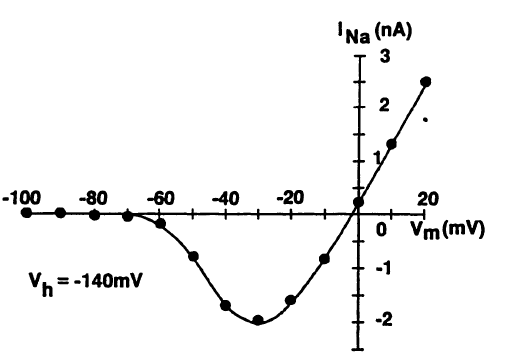
\includegraphics[width=\linewidth]{figures/IVCurveSaka.png}
        \caption{IV peak curve, figure 1B from Sakakibara \cite{Sakakibara1992}}
    \end{subfigure}
    \begin{subfigure}[b]{0.49\textwidth}
    \centering
        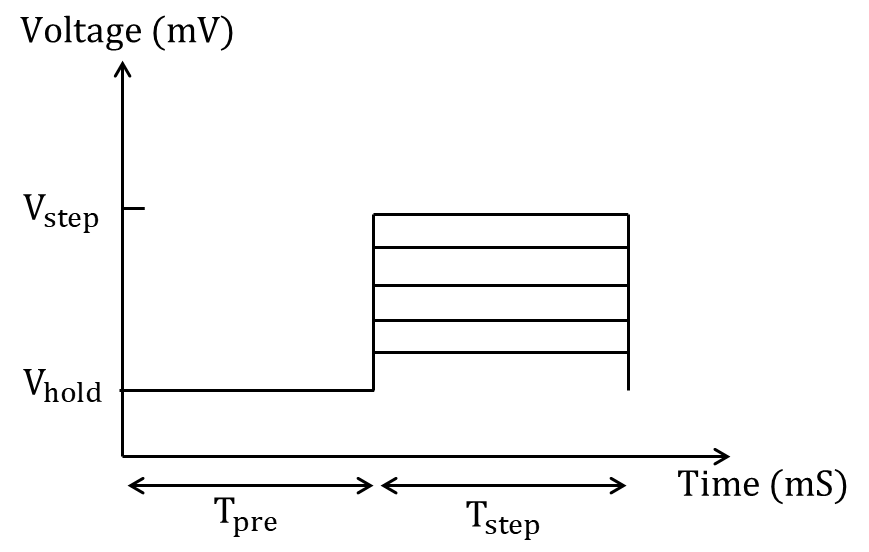
\includegraphics[width=\linewidth]{figures/SimplePulseProtocol.png}
        \caption{Example of a simple pulse protocol}
    \end{subfigure}

    ~
    \caption{IV peak experiment from Sakakibara \cite{Sakakibara1992} on left and the corresponding simple pulse protocol on the right}
    \label{fig:IVexpSaka}
\end{figure}


\subsection{Activation}

This experiment is very similar to the IV peak : a simple pulse protocol is used and the maximum absolute (peak) value of the normalized conductance ($g_{normalized} = m^3h$) is then recorded. The goal of this experiment is to measure how "activated" is the activation gate, $g_{normalized} = 1$ being activated and $g_{normalized} = 0$ not activated since during a short time the inactivation gate is still equal to 1. In this experiment the two variables of interest are therefore $g_{normalized}$ as well as $V_{step}$. Figure \ref{fig:InactCurveSaka}.a shows the conductance curve of the sodium channel ($N_{a}$) from the Sakakibara \cite{Sakakibara1992} paper (curve on the right $g_{Na}/g_{Na,max}$)

\subsection{Inactivation}

This experiment is different from the two previous in the sense where it uses a double pulse protocol : a first voltage step at $V_{step}$ is applied to the cell to inactivate it at a certain level, and another step is applied just after the first one, this time at the voltage $V_{test}$. The first pulse is long enough so the gate $h$ starts decreasing from 1 to $h_{\infty}(V_{step})$ and the purpose of the second pulse is to trigger an action potential to measure again the normalized conductance of the cell ($g_{normalized}$). This measure represent the level of inactivation of the cell previously achieved with $h_{\infty}(V_{step})$.

In real experiments, there is often a waiting time $t_{wait}$ of $2$ ms between the two voltage steps but since the voltage doesn't have the time to go back to $V_{hold}$ during this short time, the numerical experiment will neglect $t_{wait}$ for the inactivation protocol only. The figure \ref{fig:InactCurveSaka}.b represent a such double pulse protocol. Figure \ref{fig:InactCurveSaka}.a shows the $h_{\infty}$ and activation curves of the sodium channel ($N_{a}$) from the Sakakibara \cite{Sakakibara1992} paper :

\begin{figure}[H]
    \centering
    \captionsetup{singlelinecheck = false, format= hang, justification=centerlast, font=footnotesize, labelsep=space}
    \begin{subfigure}[b]{0.49\textwidth}
    \centering
        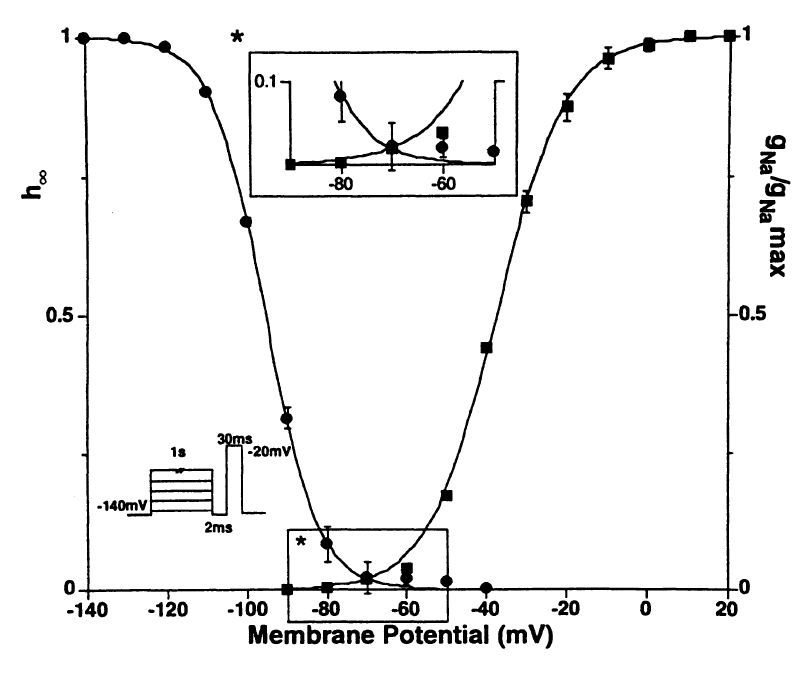
\includegraphics[width=\linewidth]{figures/InactCurveSaka.png}
        \caption{Inactivation curve (the $h_{\infty}$ curve on the left), activation curve on the right, figure 7 from Sakakibara \cite{Sakakibara1992}}
    \end{subfigure}
    \begin{subfigure}[b]{0.49\textwidth}
    \centering
        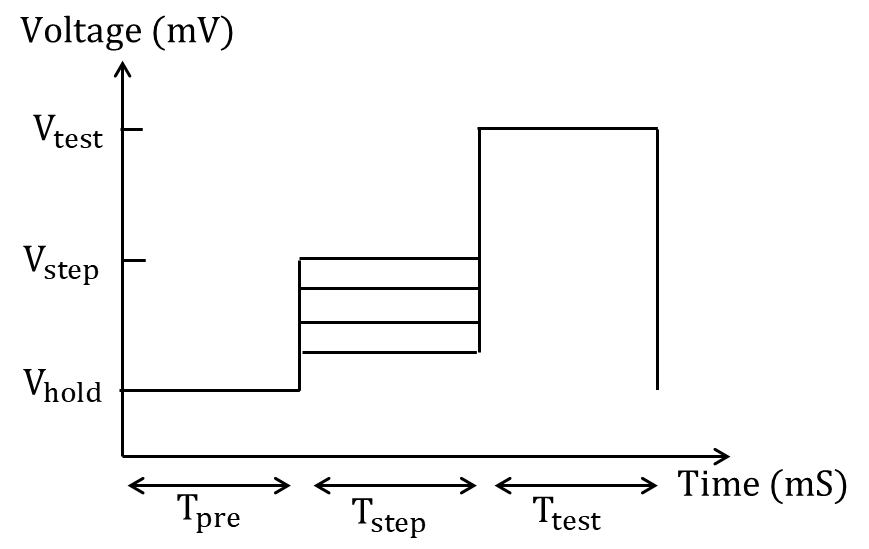
\includegraphics[width=\linewidth]{figures/InactVoltageSteps.png}
        \caption{Example of a double pulse protocol without $t_{wait}$. {\color{white} mmmmmmm } }
    \end{subfigure}

    ~
    \caption{Inactivation experiment from Sakakibara \cite{Sakakibara1992} on left and the corresponding double pulse protocol on the right}
    \label{fig:InactCurveSaka}
\end{figure}


\subsection{Time constants, Inactivation kinetics}

This experiment uses a simple pulse protocol to trigger an action potential in the cell, then a bi-exponential function ($f(t) = Ae^{-t / \tau_{f}} + Be^{-t / \tau_{s}}$) is fitted to the inactivation part of the current (Figure \ref{fig:InactKinetics}.b). The measure here is the two time constants $\tau_{h,f}$ and $\tau_{h,s}$ (f for fast; s for slow) and the point of this protocol is to measure how quickly the cell inactivates. The common orders of magnitude give $\tau_{s} \approx 5 $ to $10 \tau_{f}$ as shown on the figure \ref{fig:InactKinetics}.a. The three variables of interest are therefore $\tau_{f}$ and $\tau_{s}$ as well as $V_{step}$. So far the model introduced had only one inactivation gate $h$ to simplify, but this kind of experiment lead to a different modeling of the inactivation : two inactivation gates, with a fast one and a slow one (the fast one being still slower than the activation gate).


\begin{figure}[H]
    \centering
    \captionsetup{singlelinecheck = false, format= hang, justification=raggedright, font=footnotesize, labelsep=space}
    \begin{subfigure}[b]{0.49\textwidth}
    \centering
        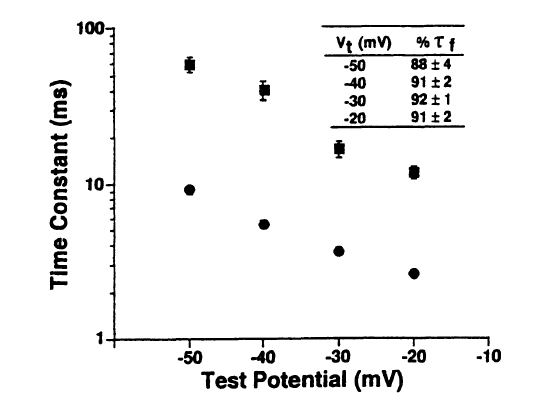
\includegraphics[width=\linewidth]{figures/SakakibaraFigure5B.PNG}
        \caption{Inactivation time constant experiment from Sakakibara \cite{Sakakibara1992}, figure 5B {\color{white} mmmmmmmmmmmmmmmmmmm }}
    \end{subfigure}
    \begin{subfigure}[b]{0.49\textwidth}
    \centering
        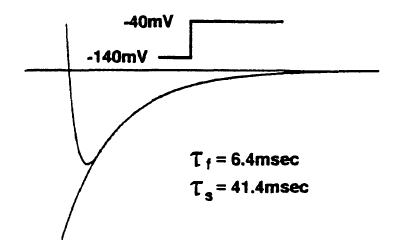
\includegraphics[width=\linewidth]{figures/InactKinSaka.png}
        \caption{A bi-exponential function, used to fit the decay phase (inactivation) of the cell, figure 5A from Sakakibara \cite{Sakakibara1992}}
    \end{subfigure}

    ~
    \caption{Inactivation time constant experiment from Sakakibara \cite{Sakakibara1992} on left and the corresponding fitting protocol on the right}
    \label{fig:InactKinetics}
\end{figure}

\subsection{Recovery}

The recovery protocol uses a double pulse protocol a bit different from the one used in the inactivation : the waiting time $T_{wait}$ between the two voltage step is not neglected anymore since it is the main part of the protocol. Indeed the protocol consists in two voltage step at $V_{test}$ with an increasing time $T_{wait}$ between both voltage steps, see figure \ref{fig:RecovSaka}.b.

The first pulse at $V_{test}$ - the conditioning pulse - fully activates the channel, which causes the activation gate to go from 0 to 1 and the inactivation gate to go from 1 to 0 at a slower rate. The value of the maximum absolute value of the current $I_{cond}$ is then recorded during this first pulse. The return to the holding potential for a varying amount of time $T_{wait}$, makes the activation gate go very quickly back to 0 (deactivation) and the inactivation more slowly back to 1 (recovery). If the inactivation gate has not returned to 1 before the second pulse, a reduced peak current output will be measured during the second pulse : this is $I_{test}$. Finally the ratio $\dfrac{I_{test}}{I_{cond}}$ is computed and represent the recovery of the channel after the inactivation during $T_{wait}$. An example of recovery experiment from Sakakibara \cite{Sakakibara1992} is shown on figure \ref{fig:RecovSaka}a .



\begin{figure}[H]
    \centering
    \captionsetup{singlelinecheck = false, format= hang, justification=centerlast, font=footnotesize, labelsep=space}
    \begin{subfigure}[b]{0.49\textwidth}
    \centering
        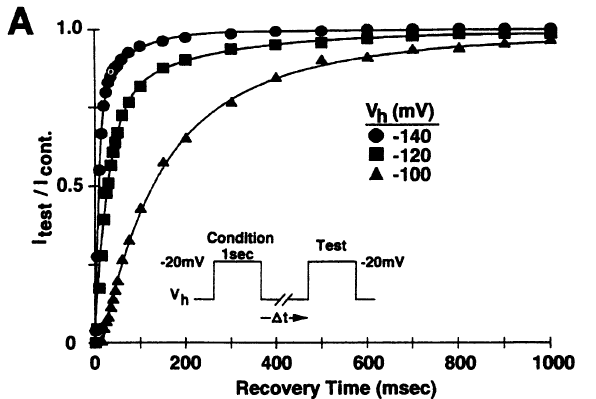
\includegraphics[width=\linewidth]{figures/RecovSaka.png}
        \caption{Recovery experiment from Sakakibara \cite{Sakakibara1992}, figure 8A {\color{white} mmmmmmm }}
    \end{subfigure}
    \begin{subfigure}[b]{0.49\textwidth}
    \centering
        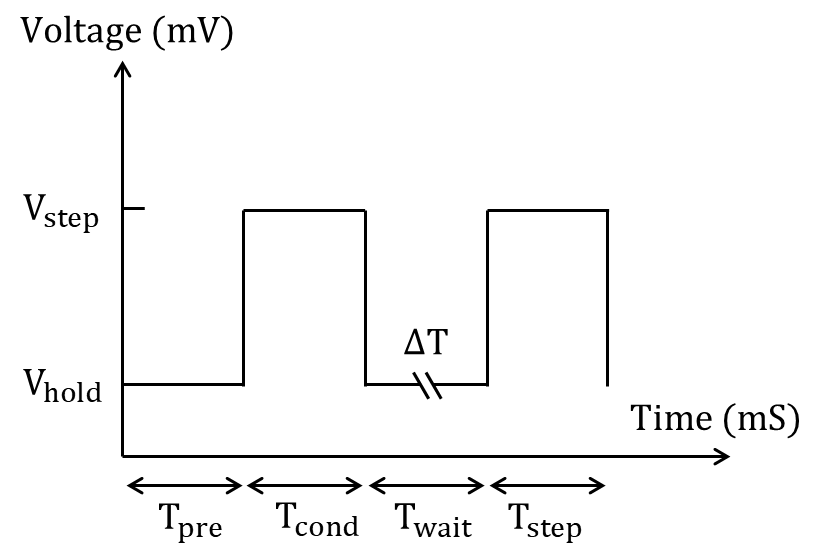
\includegraphics[width=\linewidth]{figures/DoublePulseProtocol.png}
        \caption{Example of a double pulse protocol, with the presence of $T_{wait}$ }
    \end{subfigure}

    ~
    \caption{Recovery experiment from Sakakibara \cite{Sakakibara1992} on left and the corresponding double pulse protocol on the right}
    \label{fig:RecovSaka}
\end{figure}

\subsection{Availability}

The availability protocol consists in a double pulse protocol where $T_{wait}$ is neglected, and the time increasing is now the duration of the conditioning pulse $T_{cond}$. Moreover the voltage step imposed during the condition pulse is not the same as the one imposed during $T_{test}$ : $V_{cond} \approx -100$ to $-80 mV$ whereas $V_{test} = -20$ mV. The point of this experiment is to measure the time at which the inactivation gate reaches it's value $h_{\infty}(V_{cond})$. The ratio $\dfrac{I_{test}}{I_{cond}}$ is computed the same way than for the recovery experiment and plotted against $T_{cond}$ (figure \ref{fig:AvailSaka}.a). The availability protocol is represented on figure \ref{fig:AvailSaka}.b.



\begin{figure}[H]
    \centering
    \captionsetup{singlelinecheck = false, format= hang, justification=centerlast, font=footnotesize, labelsep=space}
    \begin{subfigure}[b]{0.49\textwidth}
    \centering
        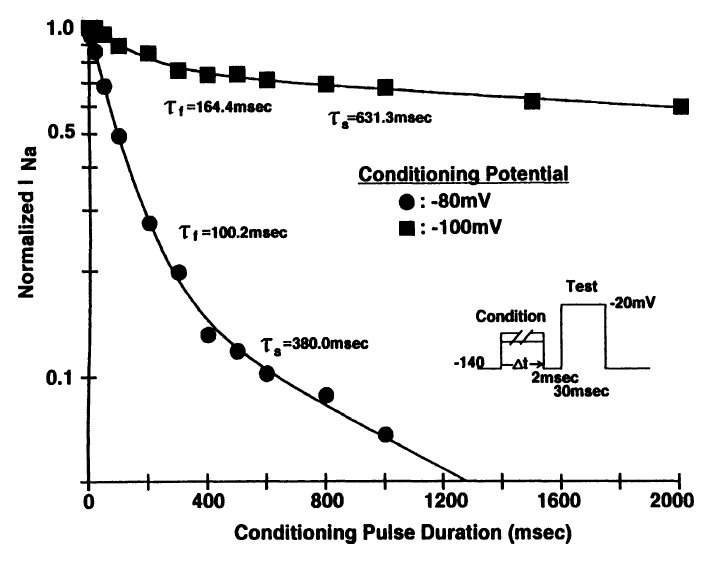
\includegraphics[width=\linewidth]{figures/AvailSaka.png}
        \caption{Availability experiment from Sakakibara \cite{Sakakibara1992}, figure 6 {\color{white} mmmmmmm }}
    \end{subfigure}
    \begin{subfigure}[b]{0.49\textwidth}
    \centering
        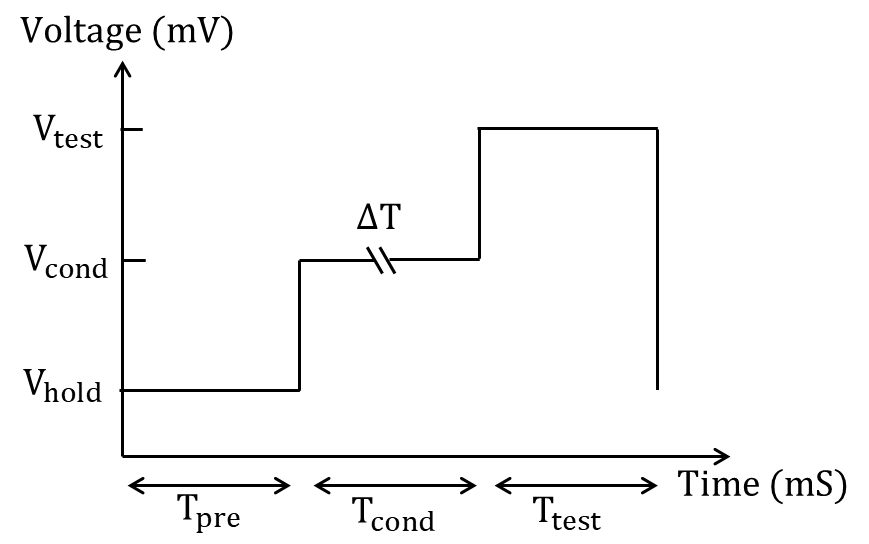
\includegraphics[width=\linewidth]{figures/AvailProtocol.png}
        \caption{Example of a double pulse protocol, without the presence of $T_{wait}$}
    \end{subfigure}

    ~
    \caption{Availability experiment from Sakakibara \cite{Sakakibara1992} on left and the corresponding double pulse protocol on the right}
    \label{fig:AvailSaka}
\end{figure}

\section{ABCSMC : Approximate Bayesian Computation Sequential Monte Carlo}

As quickly broach in the abstract, the statistical/machine learning algorithm used in the project was the Approximate Bayesian Computation, or more precisely a variant of the ABC : the "sequential Monte Carlo" variant (ABCSMC). Before explaining the algorithm itself, having a look at the following formula (Eq 2.2) will help to understand the necessity of using the ABCSMC. According to Bayes formula (Eq 2.2) the posterior $\mathbb{P}(\theta | \mathcal{D})$ distribution can be computed, where $\theta$ denotes the parameters vector, $\mathcal{D}$ the observational data, $\mathbb{P}(\mathcal{D} | \theta)$ the likelihood and $\mathbb{P}(\theta) $ the prior.
\begin{eqnarray}
\mathbb{P}(\theta | \mathcal{D}) = \dfrac{\mathbb{P}(\mathcal{D} | \theta) \mathbb{P}(\theta) }{\mathbb{P}(\mathcal{D})} 
\end{eqnarray}
The global goal of finding the optimal value of the vector parameter and its component distribution as well as variances (the uncertainty around the parameters values) reduces to finding the posterior $\mathbb{P}(\theta | \mathcal{D})$. Indeed, this is the probability of $\theta$ knowing the data set $\mathcal{D}$. The only problem here is that the model is a continuous model and that the density function $f_{\theta}(x)$ of this one is unknown. Therefore computing the likelihood $\mathbb{P}(\mathcal{D} | \theta)$ is not possible. Since this method doesn't work here, the posterior must be computed using another formula and here comes the utility of the ABCSMC : the goal of this algorithm is to estimate the posterior distribution without computing the likelihood function. The ABCSMC is in fact an iterative rejection sampler : at each iteration it samples a population of $\theta_i$ from the prior and reject all the $\theta_i$ that leads to simulated data too far from the experimental data gathered. Now, to fully understand, the ABCSMC works the following way : 

The initialisation consists in choosing an initial prior $\mathbb{P}(\theta_{0})$, a value of $\epsilon_{0}$ which will define the first distance threshold, a distance function $d$ on a vector space described afterwards and the sampled population size $N$. For the project, the prior was always chosen uniformly between two bounds for each parameter, thus defining a vector space (different from the one on which the distance function is defined), and the distance function chosen was the $L_2$ norm. 
Moreover $\epsilon_{0}=20$ and $N = 10 000$ were chosen. Finally the experiment that are going to be simulated are chosen and the experimental data of the results defines $\mathcal{D}$.

Then the algorithm chooses one vector -a particle- noted $\theta^{*}$ into the vector space defined by the prior (randomly since the initial prior is uniform). The experiments chosen are then simulated using myokit \cite{Clerx2016}, a library coded in python for simulating cardiac myocytes which are cardiac cells that can contract when electrically stimulated. After the simulation, the summary of all the simulated data is collected to form  $\mathcal{D}(\theta^{*})$ which is called the summary statistics. Using the predefined distance function $d$, the distance between $ \mathcal{D}^{*}$ ($= \mathcal{D}(\theta^{*})$) and $\mathcal{D}$ is computed: if $d(\mathcal{D}^{*},\mathcal{D}) < \epsilon_0 $ the particle $\theta^{*}$ is accepted, otherwise it is rejected. Once $N$ particles have been accepted, the first iteration of the algorithm stops and the $N$ accepted particles define the posterior $\mathbb{P}(\theta | d(\mathcal{D}^{*},\mathcal{D}) < \epsilon_0)$. Now $\epsilon_1$ is defined to be proportionally less than actual distance $d(\mathcal{D}^{*},\mathcal{D})$ that is known to be strictly less than $\epsilon_0$ : $\epsilon_1 = \alpha d(\mathcal{D}^{*},\mathcal{D}) < \epsilon_0$ with $\alpha < 1$. Then the prior is updated to take into account the posterior $\mathbb{P}(\theta | d(\mathcal{D}^{*},\mathcal{D}) < \epsilon_0)$. This defines the first iteration of the algorithm that will now choose particles for the next iteration from the updated prior that is no longer uniform.

Through the iterations, a sequence of $(\epsilon_i)_{i \in \mathbb{N}}$ is defined such as $\epsilon_{1}>\epsilon_{2}>..>\epsilon_{T}$ and since $\epsilon_{i} > 0$, that means that the sequence $(\epsilon_i)_{i \in \mathbb{N}}$ converges towards $\epsilon_{\infty}$. If $\epsilon_{\infty}$ is close to 0 (around 0.1), then $\mathcal{D}^{*}$ will converge towards $\mathcal{D}$ and the posterior will be the distribution representing the experimental data : $d(\mathcal{D}^{*},\mathcal{D}) \rightarrow 0$. Yet, if $\epsilon_{\infty}$ is too high (usually around 1) the simulated data will be far away from the experimental data. If the sequence $(\epsilon_i)_{i \in \mathbb{N}}$ has been close to $\epsilon_{\infty}$ for several iteration already, the posterior is very likely to be highly constrained meaning that the algorithm is either stuck in a bad local optima or either that the model is actually not able to reproduce the data no matter what vector parameter $\theta$ is chosen.

This convergence issue has not been treated in the scope of the project, only the sampled population size $N$ was taken into account since the limitations were imposed as computational limitations : a computation for one experiment on a population size of 10000 takes already 5 hours to run approximately and the computation was performed on the servers of Imperial College London. The size $N$ was chosen to be closest one to $2^m$, or 10000 if $2^m$ was superior to 10000, $m$ being the size of the vector parameter $\theta$. The reasoning behind this theoretical formula is that if one wants to sample the vector space of $m$ dimension with 2 values per dimension, one will need $2^m$ vectors. This would assume that the $m-1$ components are kept unchanged and that only one is changed at a time. If one wants to sample the vector space with $k$ points in each dimension, one would then need $k^m$ vectors : the curse of dimensionality appears in this problem (the computational cost increase exponentially with the number of parameters). For instance, the Nygren \cite{Nygren1998} model has 16 parameters in the sodium channel, which would give $N = 2^{16} = 65536$. However, it is important to keep in mind that the vectors are chosen according to the prior and that in practice the algorithm doesn't choose the vectors by changing one component at a time so this theoretical formula is only theoretical and would need to be checked. In order to simplify the computation, $N=10000$ was therefore chosen most of the time and an assumption was made : if the sequence of $(\epsilon_i)_{i \in \mathbb{N}}$ converges to $\epsilon_{\infty}>1$ during the iterations of the algorithm and that the posterior is highly constrained, that means that the model is actually not able to reproduce the data and not that the algorithm is stuck in a bad local optima. 


\chapter{Results}

\section{$I_{Na}$ Channel (Sodium)}

\subsection{Sakakibara \cite{Sakakibara1992} data}

Data for the six experiments previously described have been gathered from Sakakibara's paper \cite{Sakakibara1992} and the experiments independently tested on the Nygren model \cite{Nygren1998}, the Courtemanche model \cite{Courtemanche1998} and the standardised model. The standardised model equations used here are expanded in the appendix 3, since this model is slightly more complex than the one used in the section 2.2 : from now on it will have two inactivation gates. The Courtemanche (Crm) \cite{Courtemanche1998} model having too much parameters (34, which represent $2^{34} \approx 1.7e^{10}$), it has been divided into 3 parts : it's 2 inactivation gates, the slow one $j$ and the fast one $h$; and the activation gate $m$. The structural identifiability will be tested here by testing independently the experiments to see if the ABCSMC can lead to parameters that make the model match to the data points from those experiments without any other constraint than the experience itself. If a such vector parameter can be found that means that the structure of the model is able to reproduce the data from the experiment, and therefore the experiment is kept for the full calibration when the parameter identifiability test will be performed. If not, that means that the model will never be able reproduce the data with even more constraints (the other experiments) and will be taken out for the model calibration.

For the recovery and availability experiment, several curves were available in the Sakakibara paper \cite{Sakakibara1992} at different values of $V_{hold}$. In order to enable a better comparison between those experiments, the recovery and availability experiment share the same voltage $V_{hold} = -100 mV$. 

The following table (Figure \ref{tab:StructuralIdentifiabilitySaka}) gathers all the results from the 3 models performing on the 6 experiments from Sakakibara \cite{Sakakibara1992}. A green tick represent a correct modeling of the experiment from the model, as explained above. A red cross represent the opposite.

\begin{figure}[H]
\centering
\captionsetup{singlelinecheck = false, format= hang, justification=centerlast, labelsep=space}
\begin{measuredfigure}
\begin{tabular}{|c|c|c|c|c|c|}
\hline
& Nygren & standardised & Crm j & Crm h & Crm m\\
\hline
IV & \cmark   &  \cmark & \cmark & \cmark & \cmark  \\
\hline
Activation &  \cmark  &   \cmark & \cmark * & \cmark * &   \cmark \\
\hline
Inactivation &  \cmark &  \cmark &  \cmark & \cmark &   \xmark \\
\hline
Time constant &  \cmark &  \cmark & \xmark & \xmark & \xmark   \\
\hline
Recovery & \xmark &  \cmark & \cmark  & \xmark &  \xmark  \\
\hline
Availability & \xmark &  \cmark & \xmark & \xmark & \xmark  \\
\hline
\end{tabular}
\caption{Structural identifiability of the experiments performed on Sakakibara data.
 \cite{Sakakibara1992}}
\end{measuredfigure}
\addtocounter{figure}{-1}
\phantomcaption
\label{tab:StructuralIdentifiabilitySaka}
\end{figure}

*The activation experiment work on the inactivation gates models (Crm h and j) because the default parameters work for the activation gate (Crm m) are correct. To higlight a failure on those experiments, it would have been necessary to run the Crm h and j after changing all the parameters of the activation gate before.

To clearly see what is a example of structural identifiability in practice, the fig \ref{fig:StructuralIdentifiabilityRecovSka} shows the recovery experiment used to test the Nygren \cite{Nygren1998} and standardised model. 

\begin{figure}[H]
    \centering
    \begin{measuredfigure}
    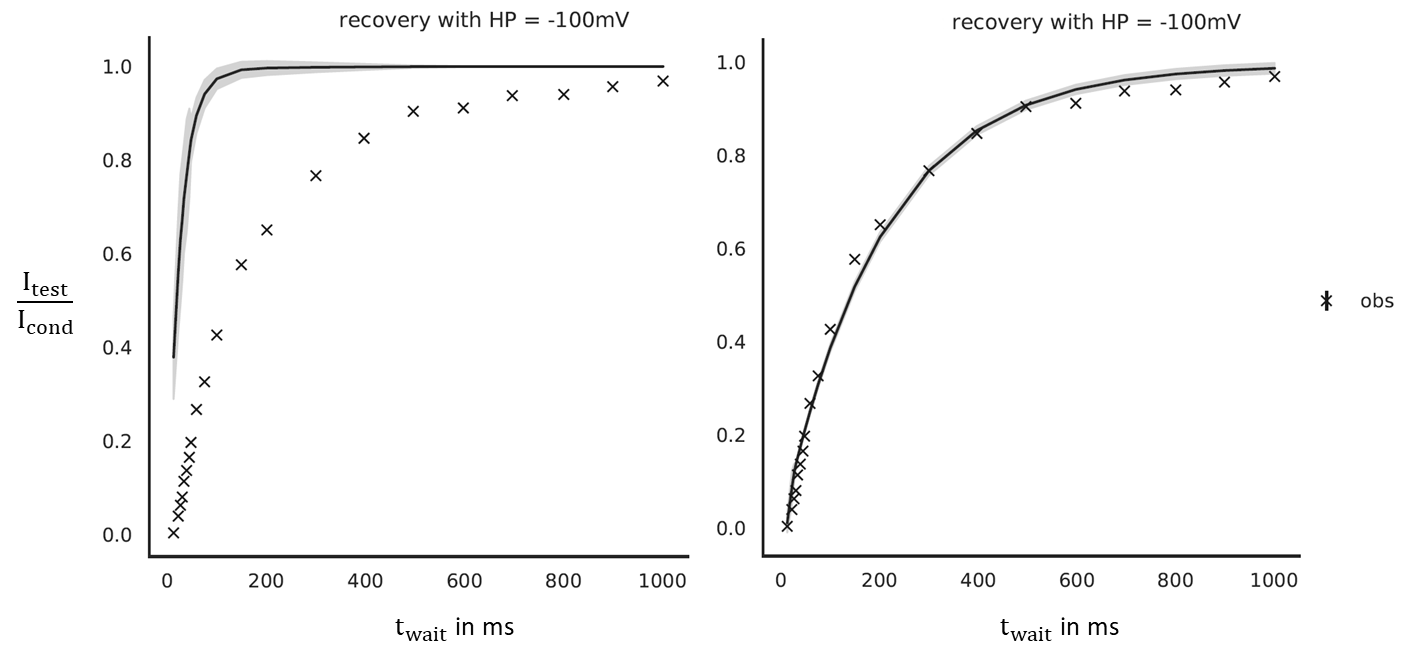
\includegraphics[width = \textwidth]{figures/structuralIdentifiabilityRecovSaka.png}
    \captionsetup{singlelinecheck = false, format= hang, justification=raggedright, font=footnotesize, labelsep=space}
    %\captionsetup{justification = centering}
	\caption{Recovery experiment for the sodium channel. On the left is the Nygren \cite{Nygren1998} model which failed the structural identifiability test. On the right is the Standardised model which succeeded in fitting the data.
}
	\end{measuredfigure}
      \addtocounter{figure}{-1}
      \phantomcaption
	\label{fig:StructuralIdentifiabilityRecovSka}
\end{figure}

Now those results allow to select which experiments will be used to calibrate the three models and in the following table (figure \ref{tab:ParameterIdentifiabilitySaka}), a "-" sign represent that the experiment X was not used to calibrate the model Y (which are represented by the red crosses in the figure \ref{tab:StructuralIdentifiabilitySaka}). For the other experiments (the green ticks in figure \ref{tab:StructuralIdentifiabilitySaka}), they will be represented by a tick if the parameter identifiability test worked : the algorithm was able to fit data from the experiment and a cross if not. The "*" on the following table represent the same particularity than on the table \ref{tab:StructuralIdentifiabilitySaka}.

\begin{figure}[H]
\centering
\captionsetup{singlelinecheck = false, format= hang, justification=centerlast, labelsep=space}
\begin{measuredfigure}
\begin{tabular}{|c|c|c|c|c|c|}
\hline
& Nygren & standardised & Crm j & Crm h & Crm m\\
\hline
IV & \cmark   &  \cmark & \cmark & \cmark & \cmark  \\
\hline
Activation &  \cmark  &   \cmark & \cmark * & \cmark * &   \cmark \\
\hline
Inactivation &  \cmark &  \xmark &  \cmark & \cmark &   - \\
\hline
Time constant &  \cmark &  \cmark & - & - & -   \\
\hline
Recovery & - &  \xmark & \cmark  & - &  -  \\
\hline
Availability & - &  \cmark & - & - & -  \\
\hline
\end{tabular}
\caption{Parameter identifiability of the experiments performed on Sakakibara data.  \cite{Sakakibara1992}}
\end{measuredfigure}
\addtocounter{figure}{-1}
\phantomcaption
\label{tab:ParameterIdentifiabilitySaka}
\end{figure}


\begin{figure}[H]
    \centering
    \captionsetup{singlelinecheck = false, format= hang, justification=centerlast, font=footnotesize, labelsep=space}
    \begin{subfigure}[b]{\textwidth}
    \centering
        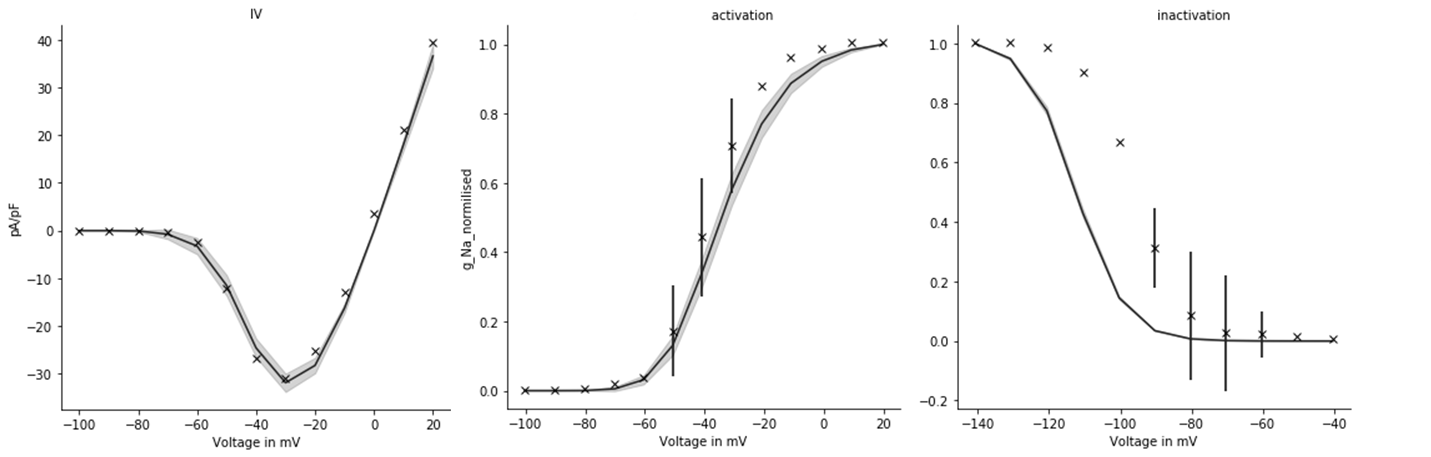
\includegraphics[width=\linewidth]{figures/Ina_Simple_saka/ina_simple_exp_iv_act_inact_all_saka_pop_10000.png}
    \end{subfigure}
    ~
    \begin{subfigure}[b]{\textwidth}
    \centering
        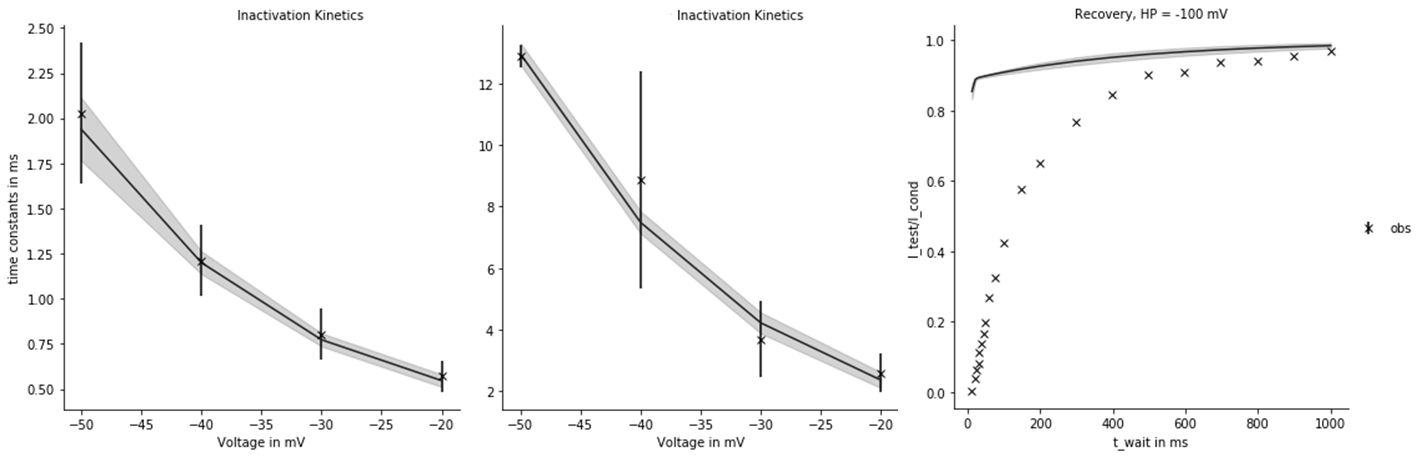
\includegraphics[width=\linewidth]{figures/Ina_Simple_saka/ina_simple_exp_inact_kin_recov_all_saka_pop_10000.png}
    \end{subfigure}
    ~
    \begin{subfigure}[b]{0.34\textwidth}
    \centering
        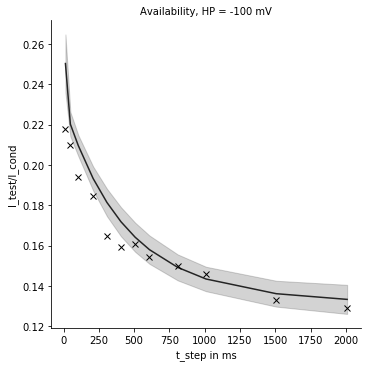
\includegraphics[width=\linewidth]{figures/Ina_Simple_saka/ina_simple_exp_availability_all_saka_pop_10000.png}
    \end{subfigure}
    ~
    \caption{Results of the parameter identifiability test for the standardised model, the grey areas correspond to the trace of the curves generated by 100 samples from the final posterior while the black line is the mean trace. The figure on the middle represent the slow inactivation time constants and the figure on its left represent the fast inactivation time constants.}
    \label{fig:resultsStandardised}
\end{figure}

On figure \ref{fig:resultsStandardised} is represented the results of the standardised model on the Sakakibara \cite{Sakakibara1992} data, when calibrating the model on all the experiments. Those results show that the recovery experiment as well as the inactivation one are not reproducible when the standardised model is constrained with the other experiments, as shown in the table \ref{tab:ParameterIdentifiabilitySaka}. The error bars on the figure \ref{fig:resultsStandardised} might seem important but those come from the variance of the data which is computed from the standard error of the mean (SEM) : $Var = sd^2 = nSEM^2$, $n$ being the number of cells on which the experiment was conducted.

On figure \ref{fig:InaPosteriorStandardSaka} one can see the posterior associated with the parameter indentifiability test ran on the standardised model. On this figure, the parameters are called $p_i$ which corresponds to $\theta_i$ in the appendix, and $p_4$ might seem to be undetermined however this is only due to the small scale of the initial prior going from 0 to $0.1$. However the parameter $p_3$ is not as constrained as the other parameters : it might be due to the fact that the equations in which $p_3$ appears, $p_1$ is also present. Yet since $p_1 >> p_3$ on the posterior distribution, that means that $p_1$ controls the activation time constant by itself and that maybe the modeling of $\tau_m$ could be simplified.

\begin{figure}[H]
    \centering
    \begin{measuredfigure}
    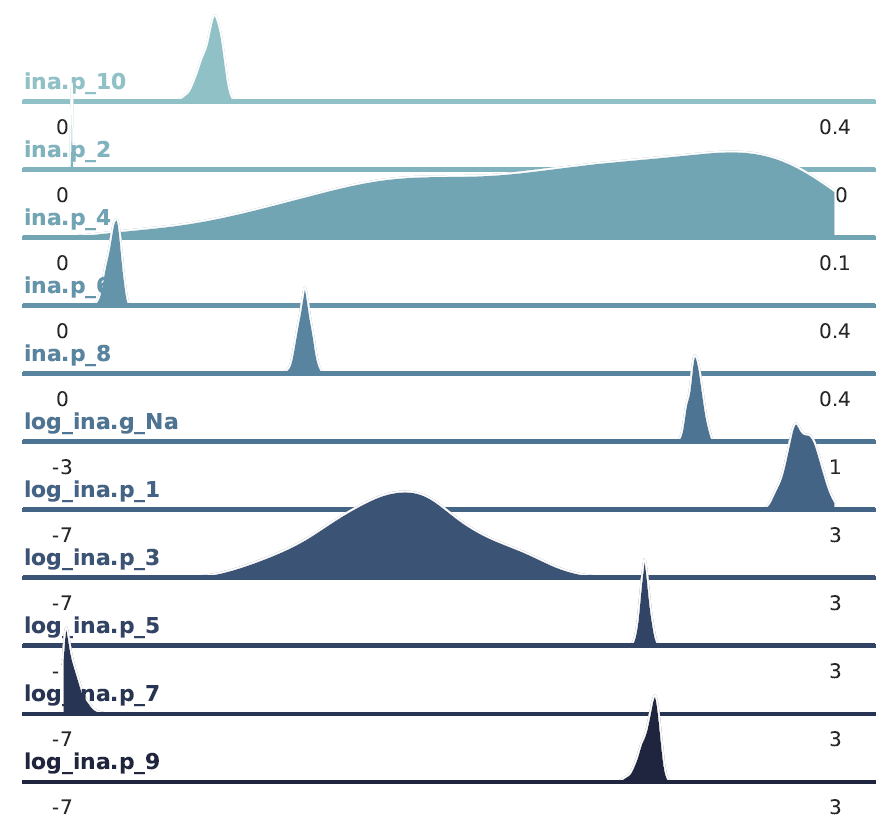
\includegraphics[scale =0.5]{figures/Ina_Simple_saka/inaStandardPosterior_all_exp_saka.PNG}
    \captionsetup{singlelinecheck = false, format= hang, justification=centerlast, labelsep=space}
    %\captionsetup{justification = justified}
	\caption{Posterior computed by the ABCSMC on the standard model using Sakakibara data \cite{Sakakibara1992}}
	\end{measuredfigure}
      \addtocounter{figure}{-1}
      \phantomcaption
	\label{fig:InaPosteriorStandardSaka}
\end{figure}

\subsection{Schneider \cite{Schneider1994} data}

This data has been collected on the Schneider \cite{Schneider1994} paper and the working experiment have been gathered here : the IV peak curve, the inactivation as well as the recovery and the availability curves. As suggested by the method workflow, the first step was to assess the structural identifiability of the 3 models (table \ref{tab:StructuralIdentifiabilitySchneider}). The parameter identifiability results of the models are summarised in table \ref{tab:ParameterIdentifiabilitySchneider}.

\begin{figure}[H]
\centering
\captionsetup{singlelinecheck = false, format= hang, justification=centerlast, labelsep=space}
\begin{measuredfigure}
\begin{tabular}{|c|c|c|c|c|c|}
\hline
& Nygren & standardised & Crm j & Crm h & Crm m\\
\hline
IV & \cmark   &  \cmark & \cmark & \cmark & \cmark  \\
\hline
Inactivation &  \cmark &  \cmark &  \cmark & \xmark &   \xmark \\
\hline
Recovery & \cmark &  \xmark & \xmark  & \xmark &  \xmark  \\
\hline
Availability & \xmark &  \xmark & \xmark & \xmark & \xmark  \\
\hline
\end{tabular}
\caption{Structural identifiability of the experiments performed on Schneider data.
 \cite{Schneider1994}}
\end{measuredfigure}
\addtocounter{figure}{-1}
\phantomcaption
\label{tab:StructuralIdentifiabilitySchneider}
\end{figure}



\begin{figure}[H]
\centering
\captionsetup{singlelinecheck = false, format= hang, justification=centerlast, labelsep=space}
\begin{measuredfigure}
\begin{tabular}{|c|c|c|c|c|c|}
\hline
& Nygren & standardised & Crm j & Crm h & Crm m\\
\hline
IV & \cmark   &  \cmark & \cmark & \cmark & \cmark  \\
\hline
Inactivation &  \cmark &  \cmark &  \cmark & - &   - \\
\hline
Recovery & \xmark &  - & -  & - &  -  \\
\hline
Availability & - &  - & - & - & -  \\
\hline
\end{tabular}
\caption{Parameter identifiability of the experiments performed on Schneider data. \cite{Schneider1994}}
\end{measuredfigure}
\addtocounter{figure}{-1}
\phantomcaption
\label{tab:ParameterIdentifiabilitySchneider}
\end{figure}

\begin{figure}[H]
    \centering
    \begin{measuredfigure}
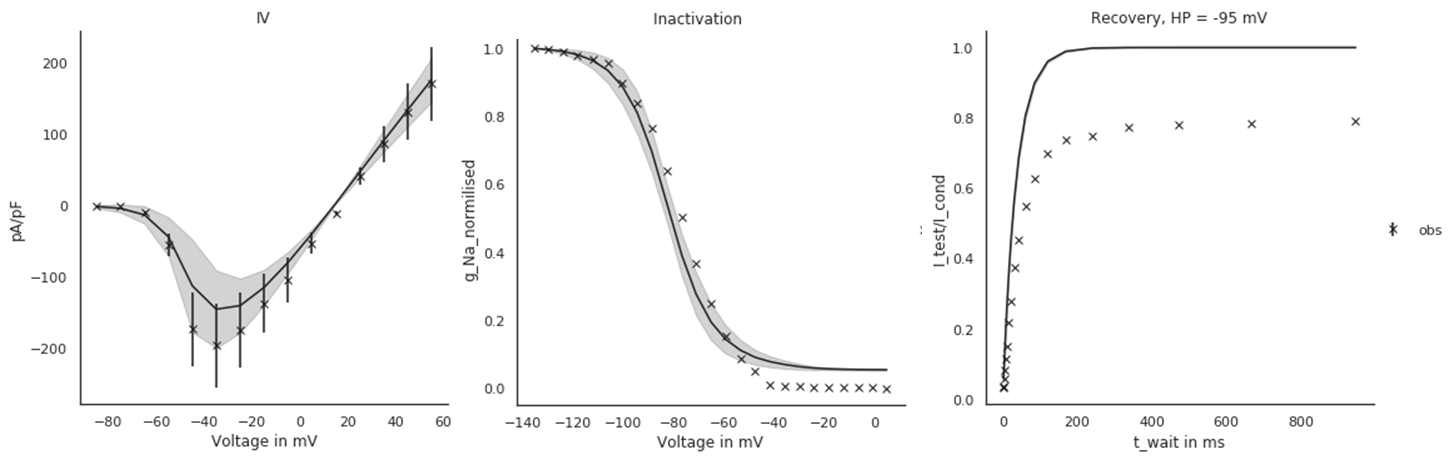
\includegraphics[width = \textwidth ]{figures/Ina_Nygren_sch/ina_nygren_exp_iv_inact_recov_all_sch_pop_10000.png}
    \captionsetup{singlelinecheck = false, format= hang, justification=centerlast, labelsep=space}
    %\captionsetup{justification = justified}
	\caption{Results of the parameter identifiability test for the Nygren \cite{Nygren1998} model, the grey areas correspond to the trace of the curves generated by 100 samples from the final posterior while the black line is the mean trace.}
	\end{measuredfigure}
      \addtocounter{figure}{-1}
      \phantomcaption
	\label{fig:InaParameterIdentifiabilityNygrenSch}
\end{figure}

\begin{figure}[H]
    \centering
    \begin{measuredfigure}
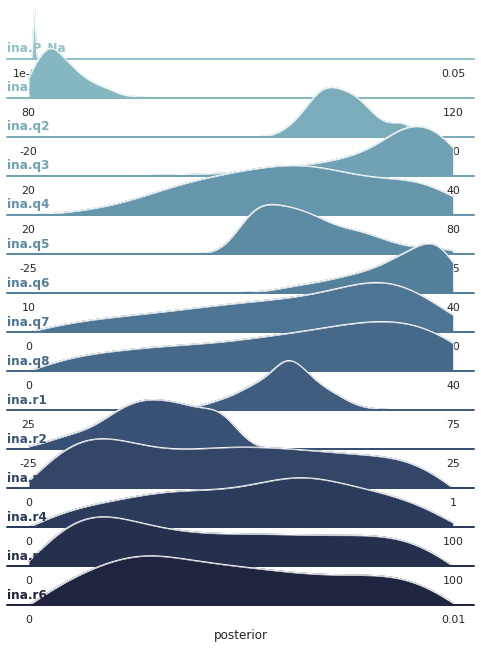
\includegraphics[scale = 0.4 ]{figures/Ina_Nygren_sch/ina_nygren_post_all_sch_pop_10000.png}
    \captionsetup{singlelinecheck = false, format= hang, justification=centerlast, labelsep=space}
    %\captionsetup{justification = justified}
	\caption{Posterior computed by the ABCSMC on the Nygren \cite{Nygren1998} model using Schneider data \cite{Schneider1994}}
	\end{measuredfigure}
      \addtocounter{figure}{-1}
      \phantomcaption
	\label{fig:InaParameterIdentifiabilityNygrenSchPost}
\end{figure}


\newpage

\section{$I_{CaL}$ Channel (Calcium)}

For this channel, only two models were tested : the Nygren \cite{Nygren1998} model and the Standard model. The data comes from Li and Nattel \cite{Li1997}, and the models were tested on the five experiments : IV, Activation, Inactivation, Time constant and Recovery. Here is the result of the modeling of those five experiments

\begin{figure}[H]
    \centering
    \captionsetup{singlelinecheck = false, format= hang, justification=centerlast, font=footnotesize, labelsep=space}
    \begin{subfigure}[b]{0.49\textwidth}
    \centering
        \begin{tabular}{|c|c|c|c|c|c|}
        \hline
        & Nygren & standardised \\
        \hline
        IV & \cmark   &  \cmark    \\
        \hline
        Activation &  \cmark  &    \cmark   \\
        \hline
        Inactivation &  \cmark &  \cmark  \\
        \hline
        Time constant &  \xmark &  \cmark  \\
        \hline
        Recovery & \cmark &  \cmark   \\
        \hline
        \end{tabular}
        \caption{Structural identifiability of the experiments performed on Li and Nattel \cite{Li1997} data.}
    \end{subfigure}
    \begin{subfigure}[b]{0.49\textwidth}
    \centering
        \begin{tabular}{|c|c|c|c|c|c|}
        \hline
        & Nygren & standardised \\
        \hline
        IV & \cmark   &  \cmark    \\
        \hline
        Activation &  \cmark  &    \cmark   \\
        \hline
        Inactivation &  \cmark &  \xmark  \\
        \hline
        Time constant &  - &  \cmark    \\
        \hline
        Recovery & \cmark &  \cmark   \\
        \hline
        \end{tabular}
        \caption{Parameter identifiability of the experiments performed on Li and Nattel data. \cite{Li1997}}
    \end{subfigure}

    ~
    \caption{Structural and parameter identifiability performed on  on Li and Nattel data. \cite{Li1997}}
    \label{fig:CaLIndentifiabilityLi}
\end{figure}

\begin{figure}[H]
    \centering
    \captionsetup{singlelinecheck = false, format= hang, justification=centerlast, font=footnotesize, labelsep=space}
    \begin{subfigure}[b]{\textwidth}
    \centering
        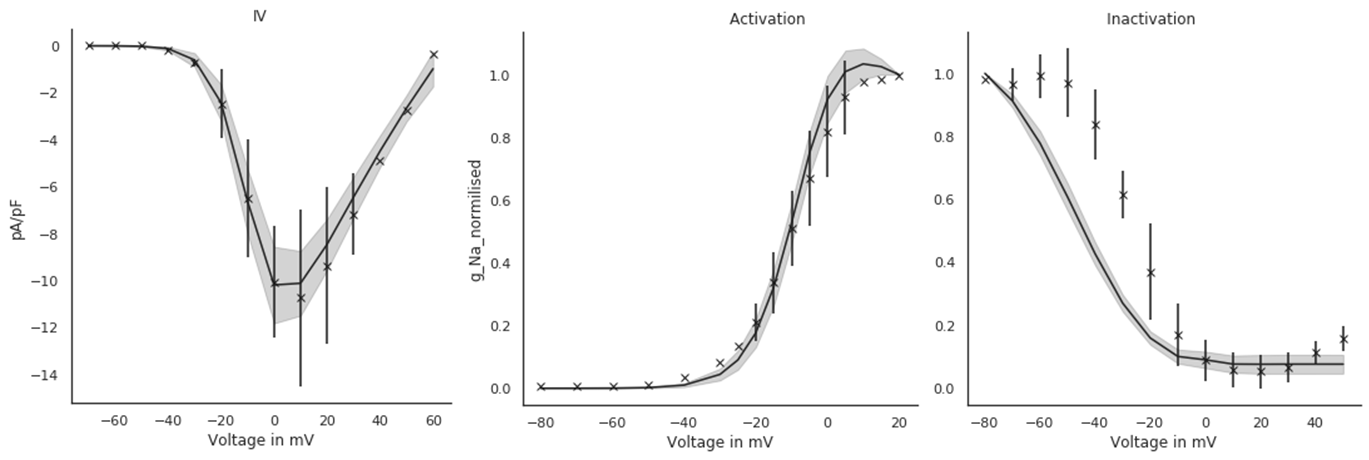
\includegraphics[width=\linewidth]{figures/Ica_Simple_Li/ica_simple_exp_iv_act_inact_all_saka_pop_10000.png}
    \end{subfigure}
    ~
    \begin{subfigure}[b]{\textwidth}
    \centering
        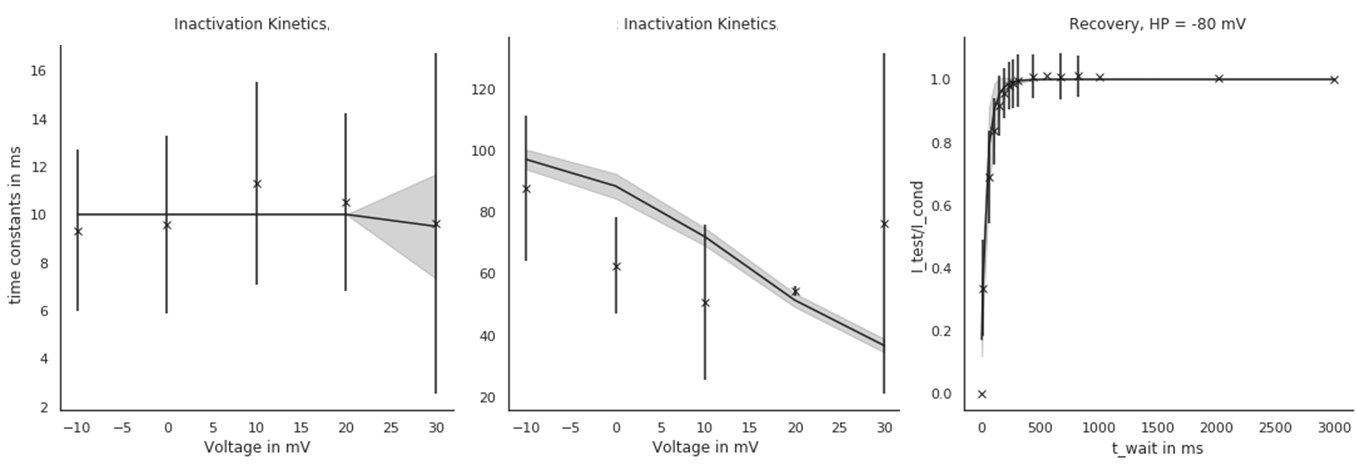
\includegraphics[width=\linewidth]{figures/Ica_Simple_Li/ica_simple_exp_inact_kin_recov_all_saka_pop_10000.png}
    \end{subfigure}
    ~

    \caption{Results of the parameter identifiability test for the standardised model, the grey areas correspond to the trace of the curves generated by 100 samples from the final posterior while the black line is the mean trace. The figure on the middle bottom represent the slow inactivation time constants and the figure on its left represent the fast inactivation time constants.}
    \label{fig:resultsStandardisedIca}
\end{figure}

\begin{figure}[H]
    \centering
    \begin{measuredfigure}
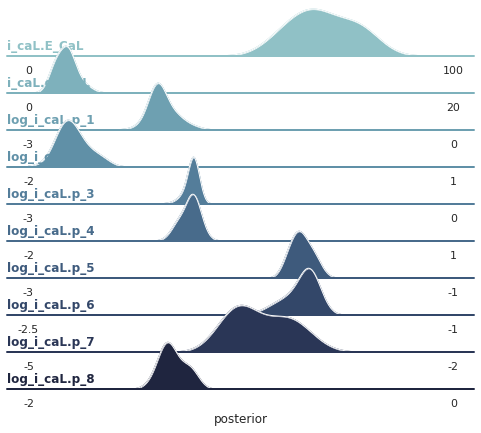
\includegraphics[scale = 0.55 ]{figures/Ica_Simple_Li/ica_simple_post_all_Li_pop_10000.png}
    \captionsetup{singlelinecheck = false, format= hang, justification=centerlast, labelsep=space}
    %\captionsetup{justification = justified}
	\caption{Results of the parameter identifiability test for the standardised model for the $I_{CaL}$ channel, the grey areas correspond to the trace of the curves generated by 100 samples from the final posterior while the black line is the mean trace.}
	\end{measuredfigure}
      \addtocounter{figure}{-1}
      \phantomcaption
	\label{fig:IcaParameterIdentifiabilityStandardLi}
\end{figure}

\chapter{Discussion}
\section{Result analysis}

\subsection{$I_{Na}$ Sakakibara \cite{Sakakibara1992}}

The first thing noticeable on the table \ref{tab:StructuralIdentifiabilitySaka} is that the only model that can structurally model all the experiments independently is also the simplest one in terms of complexity and that is the standardised model. On the other hand, the Nygren \cite{Nygren1998} model fails to catch the time changing experiments which are the recovery and the availability experiments. Yet those two experiments indirectly test the inactivation gates, which means that the structure of the inactivation gates does not fit to those experiments. However the figure \ref{fig:StructuralIdentifiabilityRecovSka} shows that $(I_{test}/I_{cond})_{simulated}$ can be approximated by a exponential function too fast for the Nygren \cite{Nygren1998} model compared to the experimental data whereas the standardised model fits to the data. The only structural difference in the inactivation gates equations between those two models is the equation of the inactivation time constants, which is coherent with the observation : the inactivation time constants modeling from the Nygren paper \cite{Nygren1998} is the reason why the model fails to reproduce the recovery and availability experiments.
On this table (\ref{tab:StructuralIdentifiabilitySaka}) one can notice that the Courtemanche \cite{Courtemanche1998} models (Crm) are coherent with the gates that they represent : the Crm j and h models which respectively represent the slow and the fast inactivation gate succeeded in modeling the inactivation experiment. The same way the Crm m fails the inactivation gate while succeeding the activation gate.

Now onto the parameter identifiability step (table \ref{tab:ParameterIdentifiabilitySaka}) : The Nygren model \cite{Nygren1998} is able to model every experiment that its structure can reproduce whereas the standardised model fails to retrieve the inactivation as well as the recovery. In fact it seems that the parameter distribution that allows the fitting of the inactivation data is close to the one that generates correctly the recovery data : it is coherent with those experimentations since they both model the inactivation gate. However the availability is also a protocol testing the inactivation gates, meaning that the parameter distribution that correctly fits the availability experiment is different from the one fitting the inactivation and recovery experiments. That would explain why the structural identifiability test did not raise any problem on the standardised model. 


\subsection{$I_{Na}$ Schneider \cite{Schneider1994}}

On the same channel but with different data, it is now the Nygren \cite{Nygren1998} model that succeeds the best to the structural identifiability test. Surprisingly it is now able to retrieve the recovery data whereas with a slightly different protocol the model could not. The difference in the time duration of the parts in the recovery protocol do not affect the result since the measure is the maximum current which is reached at the beginning of the pulse (see section 2.3.5 for more details). The difference comes from the modeling of the $I_{Na}$ current (see appendix 4), the external conditions and the dataset. 

Indeed the datasets are quite different (fig \ref{fig:RecoveryDataComparison}) : one can clearly see that the Schneider \cite{Schneider1994} data points form a exponential with a small time constant whereas the Sakakibara \cite{Sakakibara1992} data can be modeled by a exponential with a greater time constant. Yet as previously seen in the figure \ref{fig:StructuralIdentifiabilityRecovSka}, the Nygren $I_{Na}$ model \cite{Nygren1998} is only able to reproduce the fast inactivation time constant curves. This explains why the Schneider \cite{Schneider1994} data is well fitted by the Nygren model \cite{Nygren1998}. However this result also shows that the standardised model is not able to reproduce a fast inactivation time constant.

\begin{figure}[H]
    \centering
    \begin{measuredfigure}
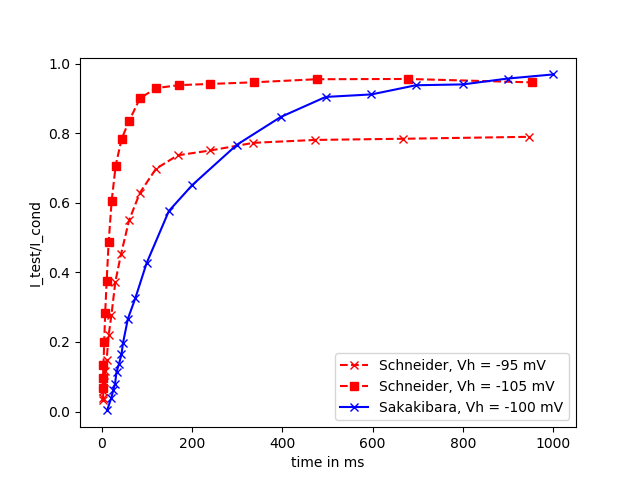
\includegraphics[scale = 0.55 ]{figures/recovdataIna.png}
    \captionsetup{singlelinecheck = false, format= hang, justification=centerlast, labelsep=space}
    %\captionsetup{justification = justified}
	\caption{Discrepencies between the Schneider \cite{Schneider1994} dataset and the Sakakibara \cite{Sakakibara1992} one for the recovery experiment. The holding potential $-100 mV$ not being available on Schneider \cite{Schneider1994} paper, the two clossest were taken : $-95 mV$ and $-105 mV$}
	\end{measuredfigure}
      \addtocounter{figure}{-1}
      \phantomcaption
	\label{fig:RecoveryDataComparison}
\end{figure}

\subsection{$I_{CaL}$ Li and Nattel \cite{Li1997}}

The remarkable thing in table \ref{tab:StructuralIdentifiabilitySchneider} is that the Nygren \cite{Nygren1998} model can retrieve the recovery experiment. The model now succeed in reproducing the recovery experiment because the modeling of the inactivation time constants for the calcium is not the same that for the sodium : the inactivation time constants equations have been changed between the two channels. However the standardised model performs still better than the Nygren one \cite{Nygren1998} when it comes to structural identifiability (fig \ref{fig:CaLIndentifiabilityLi}.a). Yet, on the figure \ref{fig:resultsStandardisedIca} which shows the results after the parameter identifiability, the standardised model fails the inactivation experiment but surprisingly succeeded in the recovery experiment. This suggests that the parameters distribution correctly modelling the inactivation is in fact different from the one correctly modelling the recovery, on the contrary to what was assumed by the results of the $I_{Na}$ channel. One possible explanation would be that the 3 parameters spaces allowing the inactivation, the recovery and the other experiments (including the availability) are disjoint.  


\section{Limitations}

The limitations of this project were mainly focused towards the computational power available and the paucity of the data. A computation on just one experiment takes a lot of time to run if the convergence is slow and that the population size $N$ is equal to 10000 : it can go up to 10 hours. This means that if the running time of the algorithm is kept reasonable (below one day) the population size has to be caped at 10000 to check the convergence hypothesis made in the section 2.4. The convergence of the algorithm being assumed is a clear limitation of this work.

This computational limitation was very penalising when assessing the Courtemanche Model \cite{Courtemanche1998} : $\theta$ had to be divided into 3 vectors parameters according to its gates $\theta_m$, $\theta_h$ and $\theta_j$. Since the parameters of the gates interact with each other, separating them might have prevented the model from performing correctly on the experiments.

Moreover, regarding the ABCSMC algorithm itself, the default parameters were left unchanged such as $\epsilon_0$. A better fit or a reduction in the cost of algorithm could have been found by tweaking those parameters.
 
Finally, the data gathered from the papers was not always precise and several hypothesis regarding the protocols had to be made for some experiments. Those paper being at least 20 years old was also a problem : there is no way to check that the protocols coded in python are indeed the ones realised experimentally. This becomes penalising when the temperature of the experiment is not given : the data is adjusted from the experimental temperature accordingly to the temperature of the model through the $Q_{10}$ factor, and any error on the temperature of the model or experiment shifts the data quite significantly.

\section{Conclusion}

In conclusion, this report shows that the existing human atrial cell models can retrieve experimental data to a certain extent : they cannot structurally retrieve all the experiments except for the standardised model but none can actually fit to all the data available at once. The standardised model reproduces the data better than the other models and with less parameters. A potential next step would be to tweak the standardised model in order to match the data at the parameter identifiability test.
Finally regarding the objectives of the project the uncertainty as well as the identifiability has been assessed on the 3 models through the project and report in the result section. 

The convergence verification needs to be checked experimentally at minima to ensure that the results are valid and to know what is the population size needed to expect the convergence of the algorithm to the global optima. One way of doing this would be to experimentally run an experiment with different population sizes to see if the parameter distribution converges after a certain population size. Because of the variance of the randomisation, that would require several runs per population size, in order to assess the mean distribution related to a certain population size.

Finding a way to keep the Courtemanche model \cite{Courtemanche1998} unseparated would also allow the correct assessment of this model.


\section{Acknowledgements}

I would like to acknowledge all my friends and family for supporting me through this year and project, as well as a special thanks to Vincianne Dewailly for everything.
I would also like to acknowledge Charlie Houston for being supportive and of very good advice as well as Chris Cantwell for accepting me into this project and leading me through the project.

\printbibliography[title={References}]



\chapter{Appendix}
\section{Appendix 1}
$$m_{\infty} = \dfrac{1}{1 + \dfrac{\theta_{3}}{\theta_{1}}exp(-(\theta_{4} + \theta_{2})V) } \; \; \; \; \; \;  \tau_{m} = \dfrac{1}{\theta_{1}exp(\theta_{2}V)+\theta_{3}exp(-\theta_{4}V)} $$
$$ h_{\infty} = \dfrac{1}{1 + \dfrac{\theta_{5}}{\theta_{7}}exp((\theta_{8} + \theta_{6})V) }  \; \; \; \; \; \;  \tau_{h} = \dfrac{1}{\theta_{5}exp(\theta_{6}V)+\theta_{7}exp(-\theta_{8}V)}$$

\section{Appendix 2}
For the time constant data (the inactivation time constant experiments) of the $I_{Na}$ channel, $Q_{10,\tau} = 2.79$ was used \cite{tenTusscher2004}. For the $I_{CaL}$ channel, $Q_{10,\tau} = 2.1$ was used \cite{tenTusscher2004}. $\alpha = -1$

For the conductance data (the IV experiment) of the $I_{Na}$ channel, $Q_{10,cond} = 1.5$ was used \cite{Correa1991}. For the $I_{CaL}$ channel, $Q_{10,cond} = 2.3$ was used \cite{Kiyosue1993}. $\alpha = 1$

\section{Appendix 3}
Here is the Standardised model for the $I_{Na}$ channel :

$h_1$ represent the fast inactivation gate and $h_2$ the slow inactivation gate.

$$I_{Na} = g_{Na}(V-E_{Na})$$
$$g_{Na} = g_{Na,max}m^{3}(Ah_1 + (1-A)h_2) $$
$$\dfrac{dm}{dt} = \dfrac{m_{\infty}(V,\theta) - m}{\tau_{m}(V,\theta)}$$
$$\dfrac{dh_1}{dt} = \dfrac{h_{1,\infty}(V,\theta) - h_1}{\tau_{h1}(V,\theta)}$$
$$\dfrac{dh_2}{dt} = \dfrac{h_{2,\infty}(V,\theta) - h_2}{\tau_{h2}(V,\theta)}$$

$$m_{\infty} = \dfrac{1}{1 + \dfrac{\theta_{3}}{\theta_{1}}exp(-(\theta_{4} + \theta_{2})V) } \; \; \; \; \; \; \tau_{m} = \dfrac{1}{\theta_{1}exp(\theta_{2}V)+\theta_{3}exp(-\theta_{4}V)} $$
$$h_{1,\infty} = \dfrac{1}{1 + \dfrac{\theta_{5}}{\theta_{7}}exp((\theta_{8} + \theta_{6})V) }
\; \; \; \; \; \; \tau_{h1} = \dfrac{1}{\theta_{5}exp(\theta_{6}V)+\theta_{7}exp(-\theta_{8}V)}$$
$$h_{2,\infty} = \dfrac{1}{1 + \dfrac{\theta_{9}}{\theta_{11}}exp((\theta_{12} + \theta_{10})V) } \; \; \; \; \; \; \tau_{h2} = \dfrac{1}{\theta_{9}exp(\theta_{10}V)+\theta_{11}exp(-\theta_{12}V)}$$

$$A = 0.9$$
$$\theta_{11} = \dfrac{\theta_{7}\theta_{9}}{\theta_{5}}$$
$$\theta_{12} = \theta_{6} + \theta_{8} - \theta_{10}$$

\section{Appendix 4}

Here is the Nygren \cite{Nygren1998} model for the $I_{Na}$ channel :

$h_1$ represent the fast inactivation gate and $h_2$ the slow inactivation gate.

$$I_{Na} = g_{Na}(V-E_{Na})$$
$$g_{Na} = g_{Na,max}m^{3}(Ah_1 + (1-A)h_2) $$
$$\dfrac{dm}{dt} = \dfrac{m_{\infty}(V,\theta) - m}{\tau_{m}(V,\theta)}$$
$$\dfrac{dh_1}{dt} = \dfrac{h_{\infty}(V,\theta) - h_1}{\tau_{h1}(V,\theta)}$$
$$\dfrac{dh_2}{dt} = \dfrac{h_{\infty}(V,\theta) - h_2}{\tau_{h2}(V,\theta)}$$

$$m_{\infty} = \dfrac{1}{1 + exp \left(\dfrac{\theta_{1} +V}{\theta_{2}}\right)} \; \; \; \; \; \; \tau_{m} = \theta_{3}exp \left( -\left(\dfrac{V + \theta_{4}}{\theta_{5}}\right) \right) + \theta_{6} $$
$$h_{\infty} = \dfrac{1}{1 + exp \left(\dfrac{\theta_{7} +V}{\theta_{8}}\right)}$$
$$\tau_{h1} = \dfrac{\theta_{9}}{1 + exp \left(\dfrac{\theta_{10} +V}{\theta_{11}}\right)} + \theta_{12} \; \; \; \; \; \; \tau_{h2} = \dfrac{\theta_{13}}{1 + exp \left(\dfrac{\theta_{10} +V}{\theta_{11}}\right)} + \theta_{14}$$

$$A = 0.9$$

$$R = 8314.0 mJ/molK$$
$$T = 306.15 K (=33°C) $$
$$F = 96487.0 C/mol$$
$$E_{Na} = \dfrac{RT}{F}log\dfrac{[N_a^+]_o}{[N_a^+]_i}$$

With $[N_a^+]_o$ the sodium concentration in the extracellular space and $[N_a^+]_i$ the sodium concentration in the intracellular space.


\end{document}
